\chapter{Evaluation}
    %
    \section{Calibration of the Force Sensor}
        Because of a measurement misfortune for the calibration, the common way for determining the calibration factor is inoperable. Therefore another method is improvised. Originally, the calibration factor $ c $ was supposed to be determined by the linear fit of the ADC result-force-curve, while the weight of the different masses would have been converted into forces:
        \begin{align}
            c=\frac{\Delta n}{\Delta F} &&\left[\frac{1}{\SI{}{mN}}\right]
        \end{align}
        Since this measurement failed, the literature value of the surface tension of distilled water has to be used in order to be able to carry out a backward calculation. For that, \cref{eq:surface tension} is transformed into the force $ F_0 $:
        \begin{align*}
            F_0=\sigma \cdot 4\pi \cdot R_{ring}
        \end{align*}
        With
        \begin{align}
            F_0=F_{max}=\frac{n_{max}}{c}
            \label{eq:force}
        \end{align}
        it follows for distilled water:
        \begin{gather}
            \frac{n_{max}}{c} = \sigma_{H_2O} \cdot 4\pi \cdot R_{ring} \nonumber \\
            \Leftrightarrow \nonumber \\
            c = \frac{n_{max}}{\sigma_{H_2O} \cdot 4\pi \cdot R_{ring}}
            \label{eq:calibration factor}
        \end{gather}
        with \(\sigma_{H_2O}=\SI{72.8}{\frac{mN}{m}}\) at \SI{20}{\celsius} \cite{Eichler.2016} and \(R_{ring} = \SI{0.03}{m} \pm \SI{0.00005}{m}\)
        (approximated with the inner radius $ r_i=\SI{0.02923}{m} $ and outer radius $ r_o=\SI{0.03}{m} $)\par\medskip
        %
        The ADC result \(n_{max}\) can be read from \textsc{Du Noüy}s ring method measurements with distilled water (\cref{fig:du_nouy_method_measurement_with_distilled_water_no_1_for_calibration}).
        There are 10 values for \(n_{max}\):
        \begin{align*}
            n_{max,i}=[80321, 77600, 77085, 80827, 76744, 82423, 79322, 77319, 79543, 77873]
        \end{align*}
        The mean value and the standard deviation are
        \begin{align*}
            \bar{n}_{max}&=78906 \\
            \Delta n_{max}&=1883
        \end{align*}
        \Cref{eq:calibration factor} gives the calibration factor with
        \begin{align*}
            \boxed{c=\SI{(2875 \pm 73)}{\frac{1}{mN}}}
        \end{align*}
        The deviation of the calibration factor is calculated as follows:
        \begin{align}
            \Delta c    &=\left| \frac{\partial c}{\partial n_{max}} \right| \cdot \Delta n_{max} + \left| \frac{\partial c}{\partial R_{Ring}} \right| \cdot \Delta R_{Ring} \nonumber \\
                        &=\frac{\Delta n_{max}}{\sigma_{H_2O} \cdot 4\pi \cdot R_{Ring}} + \frac{n_{max} \cdot \Delta R_{Ring}}{\sigma_{H_2O} \cdot 4\pi \cdot R_{Ring}^2} \nonumber \\
                        &=\frac{1883}{\SI{72.8}{\frac{mN}{m}} \cdot 4\pi \cdot \SI{0.03}{m}} + \frac{78906 \cdot 5 \cdot \SI{10^{-5}}{m}}{\SI{72.8}{\frac{mN}{m}} \cdot 4\pi \cdot (\SI{0.03}{m})^2} \nonumber \\
                        &=\SI{68.61}{\frac{1}{mN}}+\SI{4.79}{\frac{1}{mN}} \nonumber \\
                        &=\SI{73.4}{\frac{1}{mN}} \approx \SI{73}{\frac{1}{mN}}
        \end{align}
        \begin{figure}[h]
            \centering
            % 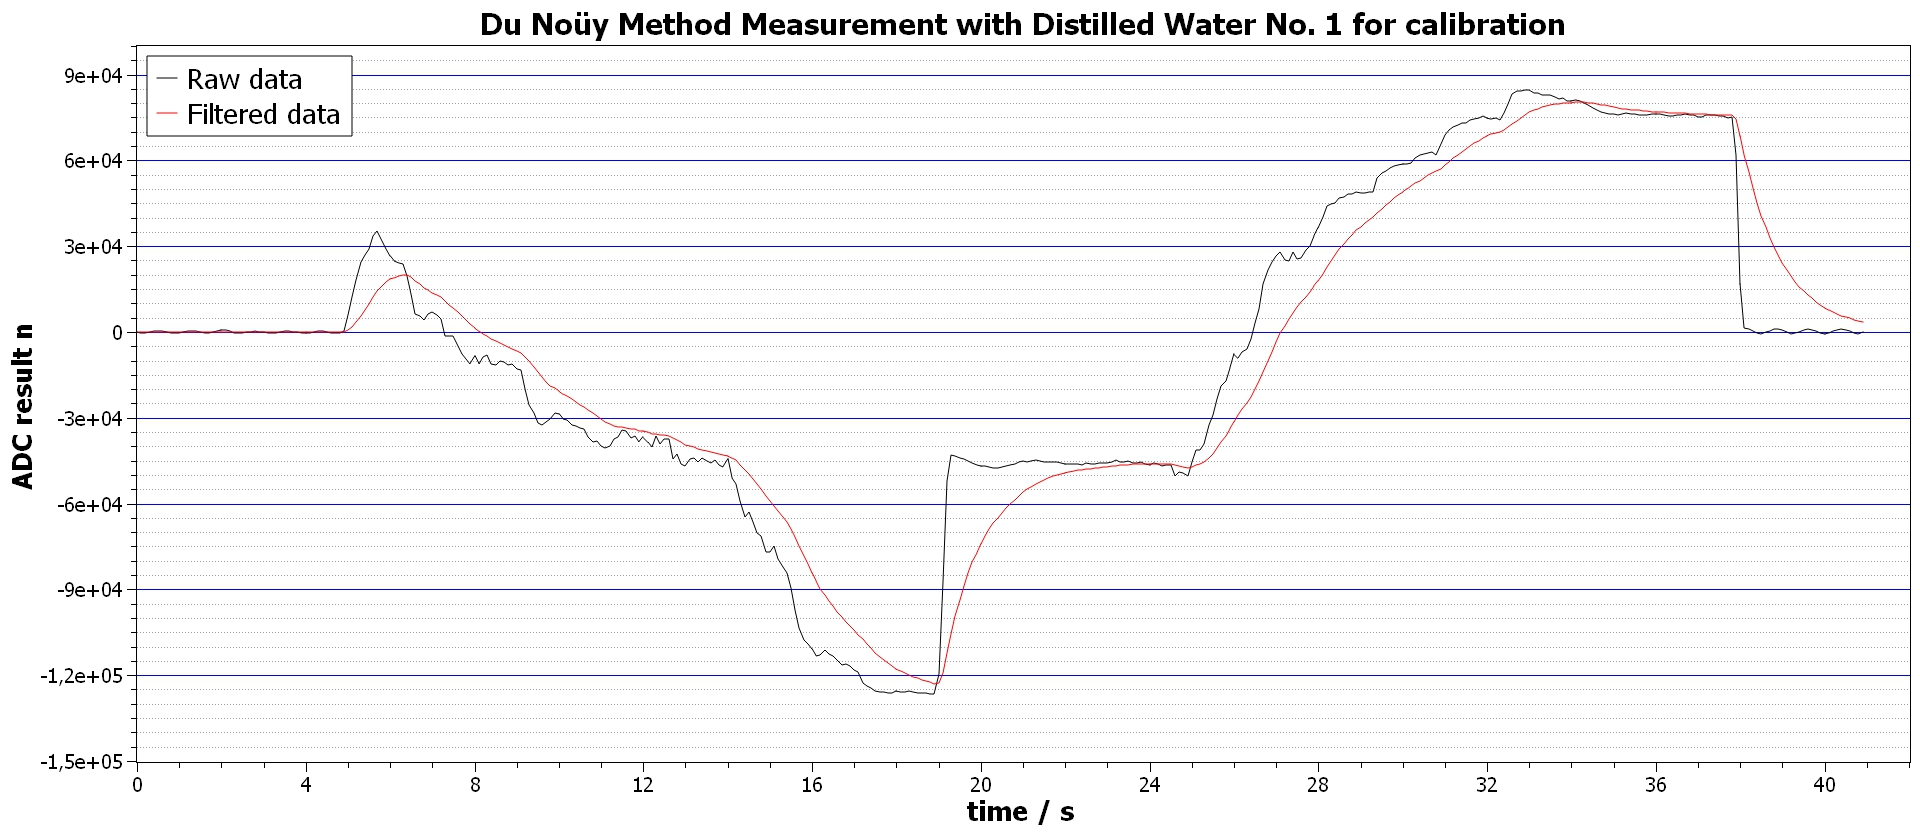
\includegraphics[width=.9\textwidth]{scidavis/Du_Nouy_Method_Measurement_with_distilled_water_No_1_for_cal.jpg}
            \includesvg[inkscapelatex=false, width=.9\textwidth]{scidavis/Du_Nouy_Method_Measurement_with_distilled_water_No_1_for_cal}
            \caption[Measurement with \textsc{Du Noüy} ring in distilled water (\(\vartheta \approx \SI{20}{\celsius}\))]{Measurement with \textsc{Du Noüy} ring in distilled water (\(\vartheta \approx \SI{20}{\celsius}\)).}
            \label{fig:du_nouy_method_measurement_with_distilled_water_no_1_for_calibration}
        \end{figure}
        %
    \section{Resolution and Statistics}
        For comparison of the raw and filtered data of the ADC with regard to statistical variations, both are
        plotted as a function of the time in a stray diagram in \cref{fig:adc_result}.\par
        As it can be seen, the raw data has a greater scattering. This is also confirmed by the standard deviations, which are as follows:
        \begin{figure}[h]
            \centering
            % 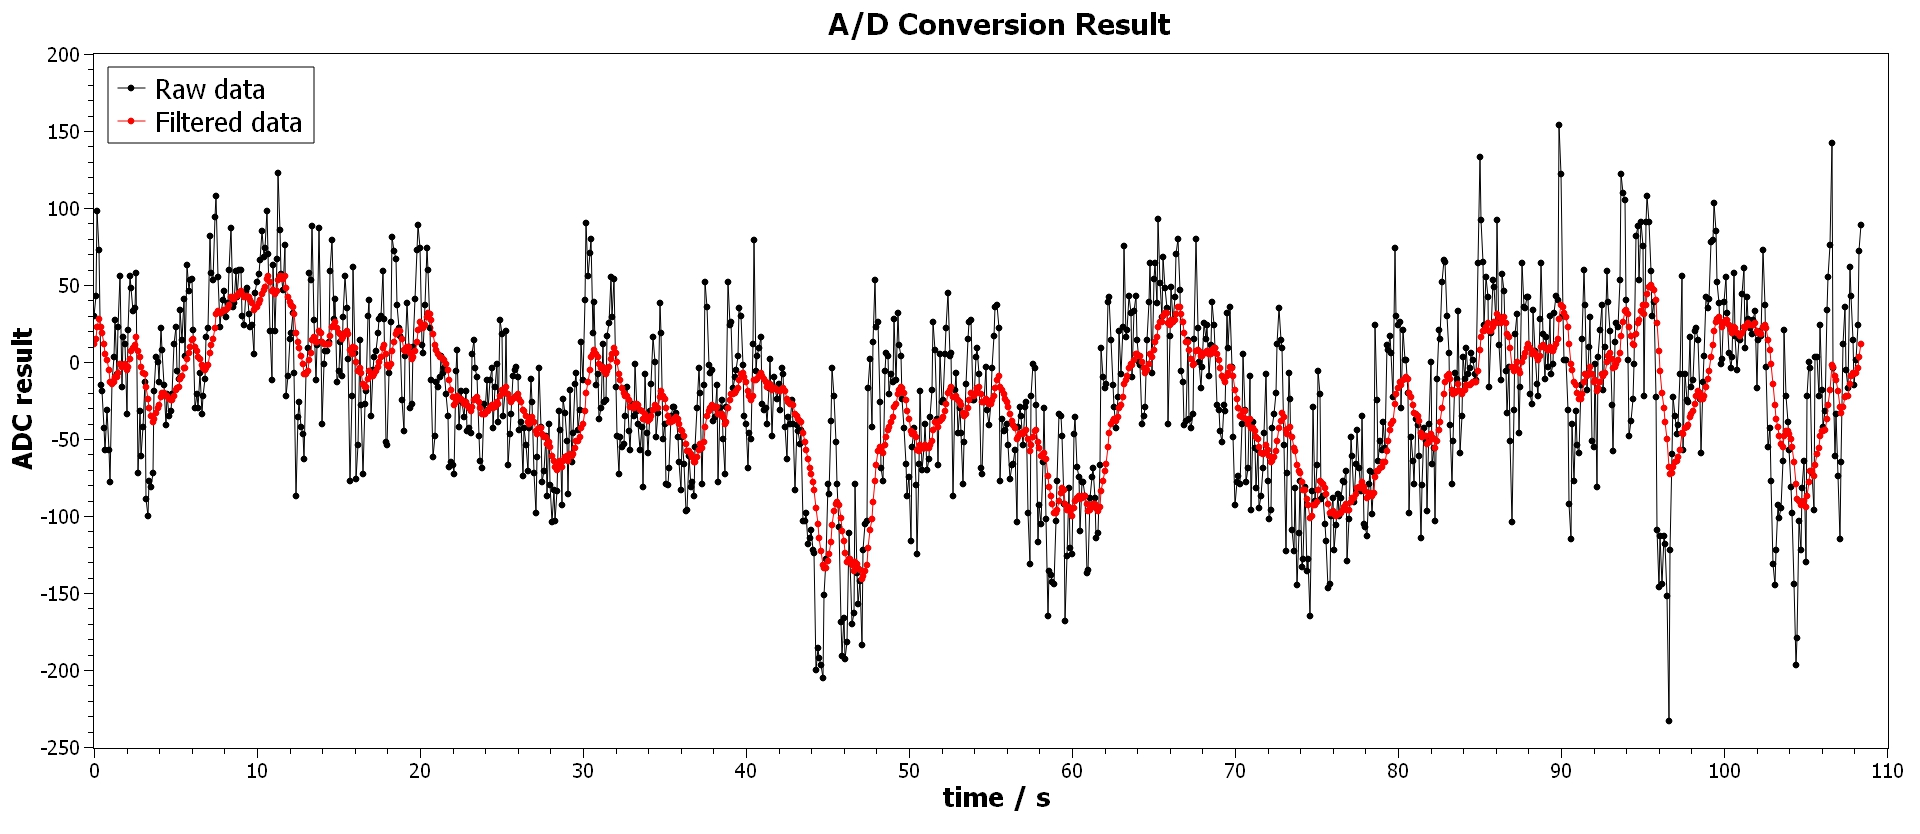
\includegraphics[width=.9\textwidth]{scidavis/ADC_result.jpg}
            \includesvg[inkscapelatex=false, width=.9\textwidth]{scidavis/ADC_result}
            \caption[Stray diagram with no load applied to force sensor]{Stray diagram with no load applied to force sensor.}
            \label{fig:adc_result}
        \end{figure}
        \begin{align*}
            \bar{n}_{raw}       &=-21 \qquad \sigma_{raw}=58\\
            \bar{n}_{filtered}  &=-23 \qquad \sigma_{filtered}=39
        \end{align*}
        Based on that, the deviation of the force to be read can be determined as
        \begin{align}
            \Delta F    &=\left| \frac{\partial F}{\partial \bar{n}_{filtered}} \right| \cdot \sigma_{filtered} + \left| \frac{\partial F}{\partial c} \right| \cdot \Delta c \nonumber \\
                        &=\frac{1}{c} \cdot \sigma_{filtered} + \frac{\left|\bar{n}_{filtered}\right|}{c^2} \cdot \Delta c \nonumber \\
                        &=\frac{39}{\SI{2875}{\frac{1}{mN}}} + \frac{23 \cdot \SI{73}{\frac{1}{mN}}}{(\SI{2875}{\frac{1}{mN}})^2} \cdot \SI{73}{\frac{1}{mN}} \nonumber \\
                        &=\SI{0.0135}{mN}+\SI{0.0002}{mN} \nonumber \\
                        &=\SI{13.7}{\micro N}
        \end{align}
        The effective resolution of the ADC is given by means of \cref{eq:ENOB}:
        \begin{align*}
            ENOB&=-23-\log_2(39)=-28
        \end{align*}
        Further, the histograms (\cref{fig:histogram_raw_data} and \cref{fig:histogram_filtered_data}) show that the raw
        data is more widely spread than the filtered one. The raw data histogram has a binning value of \(\approx 40\) while the
        filtered datas binning value is \(\approx 20\).\par\medskip
        \begin{figure}[h]
            \centering
            % 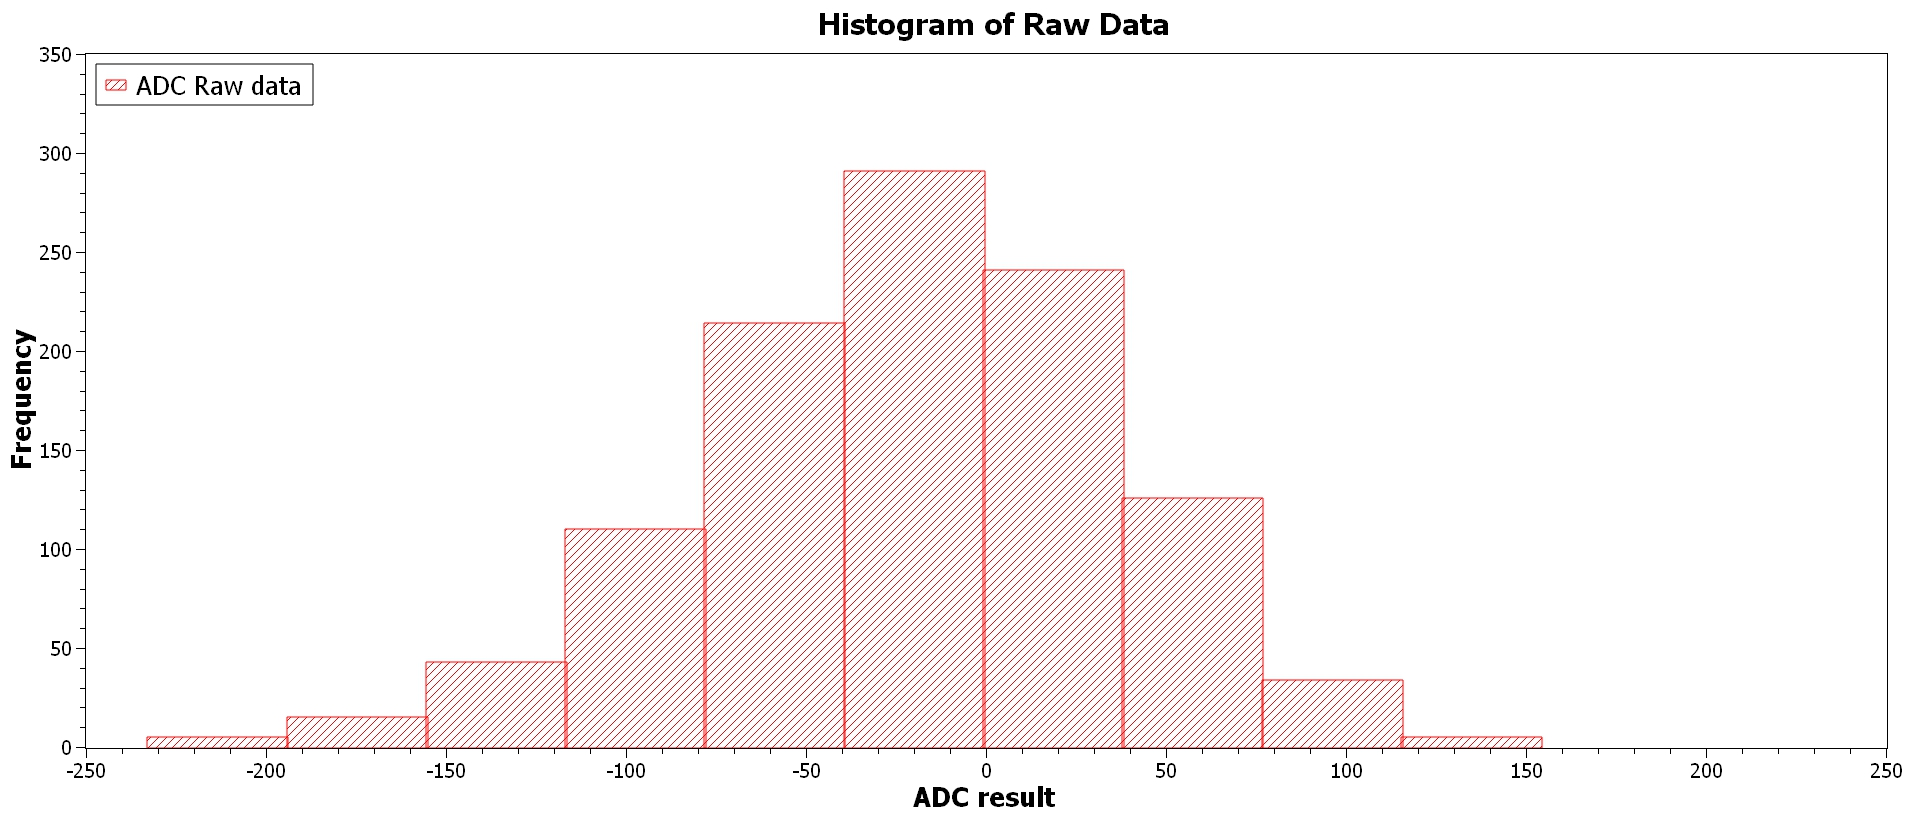
\includegraphics[width=.9\textwidth]{scidavis/histogram_raw_data.jpg}
            \includesvg[inkscapelatex=false, width=.9\textwidth]{scidavis/histogram_raw_data}
            \caption[Histogram of raw data]{Histogram of raw data.}
            \label{fig:histogram_raw_data}
        \end{figure}
        
        \begin{figure}[h]
            \centering
            % 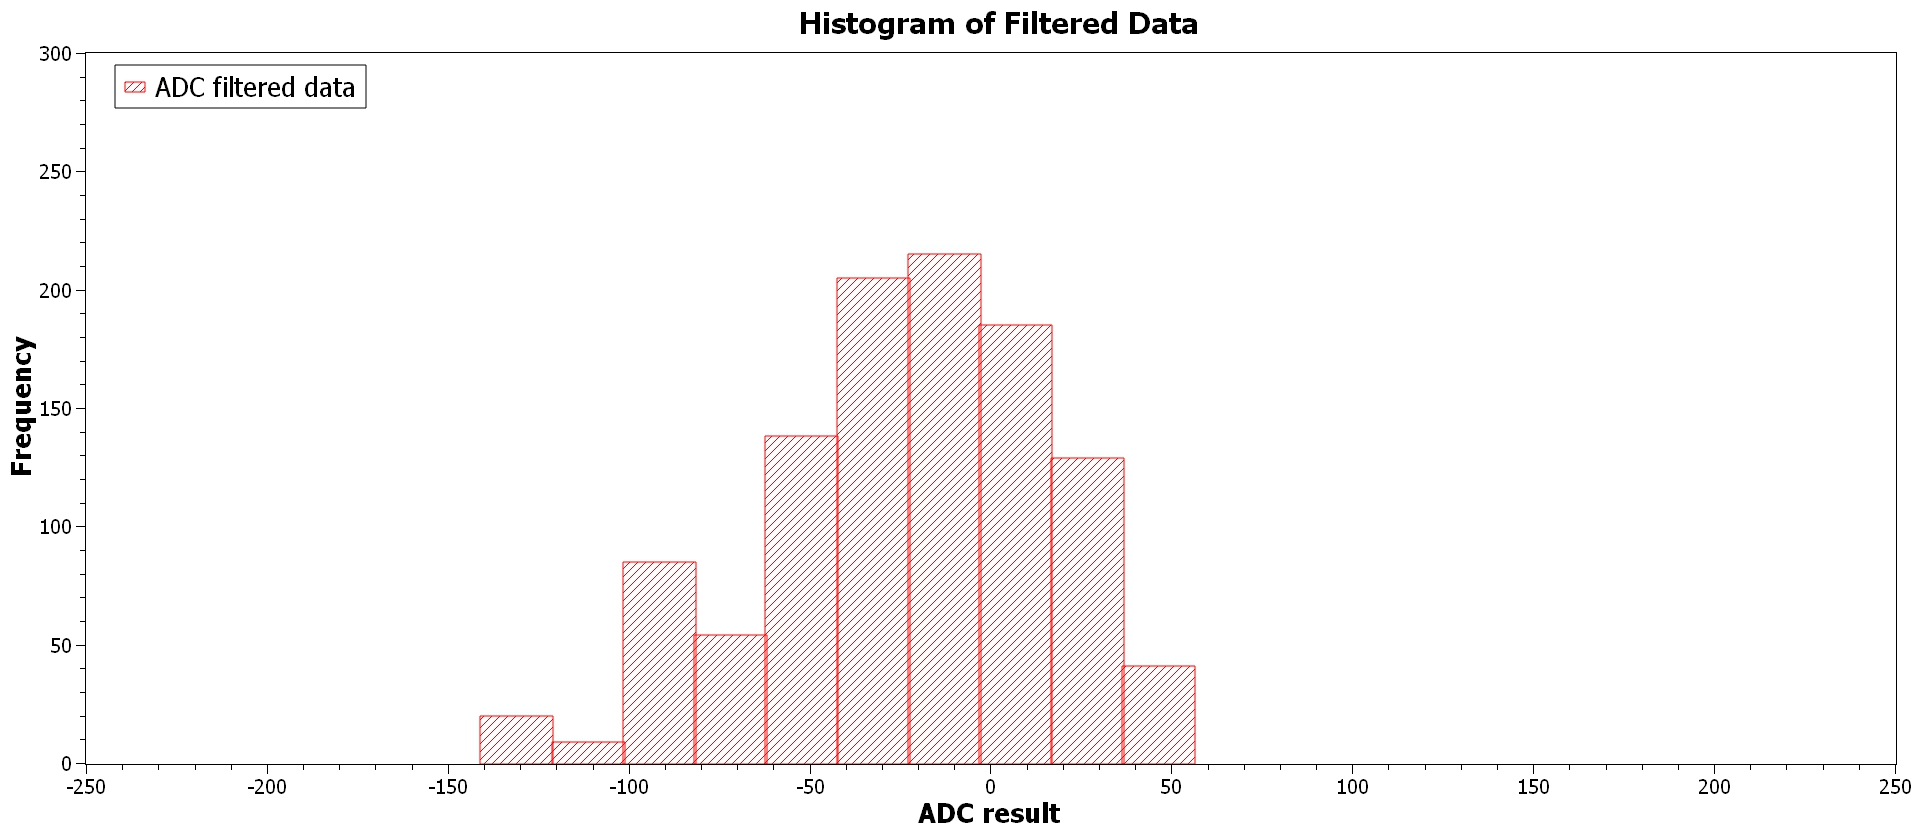
\includegraphics[width=.9\textwidth]{scidavis/histogram_filtered_data.jpg}
            \includesvg[inkscapelatex=false, width=.9\textwidth]{scidavis/histogram_filtered_data}
            \caption[Histogram of filtered data]{Histogram of filtered data.}
            \label{fig:histogram_filtered_data}
        \end{figure}
        %
    \section{\textsc{Du Noüy} Ring Method Measurement}
        The data is being sent to the PC during the measurement procedure. The diagram representing force over time, as it
        is displayed in \cref{fig:Du_Nouy_Method_Measurement_with_distilled_water_No_1,fig:Du_Nouy_Method_Measurement_with_detergent_No_1,fig:Du_Nouy_Method_Measurement_with_more_detergent_No_1,fig:Du_Nouy_Method_Measurement_with_isopropanol_No_1}, is obtained converting the ADC data into the force by way of \cref{eq:force}. 
        %
        \subsection{Distilled Water}
            The maximum forces for distilled water are as follows:
            \begin{align*}
                F_{max,i}^{H_2O}=[27.9, 27.0, 26.8, 28.1, 26.7, 28.7, 27.6, 26.9, 27.7, 27.1] && [\SI{}{mN}]
            \end{align*}
            The forces are around the mean value
            \begin{align*}
                \bar{F}_{max}^{H_2O}=\SI{(27.5 \pm 0.7)}{mN}
            \end{align*}
            so the calculated value in \cref{eq:calculated force} is approximated well. By using \cref{eq:surface tension}
            for the surface tension of distilled water, it results:
            \begin{align*}
                \boxed{\sigma_{H_2O}^{det}=\SI{(72.95 \pm 0.15)}{\frac{mN}{m}}}
            \end{align*}
            with a deviation
            \begin{align}
                \Delta \sigma_{H_2O}^{det}  &= \left| \frac{\partial \sigma_{H_2O}^{det}}{\partial \bar{F}_{max,H_2O}} \right| \cdot \Delta F + \left| \frac{\partial \sigma_{H_2O}^{det}}{\partial R} \right| \cdot \Delta R \nonumber \\
                                            &= \frac{\Delta F}{4\pi \cdot R_{ring}} + \frac{\bar{F}_{max}^{H2O}\cdot \Delta R_{ring}}{4\pi \cdot R_{ring}^2} \nonumber \\
                                            &= \frac{\SI{0.01}{mN}}{4\pi \cdot \SI{0.03}{m}} + \frac{\SI{27.5}{mN}}{4\pi \cdot (\SI{0.03}{m})^2} \cdot \SI{0.00005}{m} \nonumber \\
                                            &= \SI{0.0265}{\frac{mN}{m}} + \SI{0.122}{\frac{mN}{m}} \nonumber \\
                                            &= \SI{148.5}{\frac{\micro N}{m}} \approx \SI{150}{\frac{\micro N}{m}}
            \end{align}
            The determined value of $ \SI{72.95}{\frac{mN}{m}} $ fits well with the literature value of $ \SI{72.8}{\frac{mN}{m}} $. The area of error covers the literature value.
            %
        \subsection{Detergent}
            The maximum forces for detergent are
            \begin{align*}
                F_{max,i}^{\rho_1} = [26.8, 25.8, 26.4, 23.9, 21.0, 21.6, 23.0, 22.6, 27.9, 23.8] &&[\SI{}{mN}]
            \end{align*}
            and their mean value is
            \begin{align*}
                \bar{F}_{max}^{\rho_1}=\SI{(24.3 \pm 2.3)}{mN}
            \end{align*}
            For the detergents surface tension it results:
            \begin{align}
                \boxed{\sigma_{\rho_1}=\SI{(64.46 \pm 0.13)}{\frac{mN}{m}}}
            \end{align}
            The deviation is calculated equivalently to the one of distilled water.\par\medskip
            %
            In order to be able to compare this value with the literature value, the concentration used has to be estimated.
            Due to lack of preceding measurements of the masses \(m_{detergent}\) of detergent applied to the water, the mass
            per application is approximated with \SI{0.01}{g}. Furthermore, the type of detergent was assumed to be sodium dodecyl sulfate
            as it is a commonly used detergent. Its molar mass \(M\) is \SI{288.4}{\frac{g}{mol}} \cite{sodium.dodecyl.sulfate.cas.entry.2021}.
            For the amount of the substance \(N\) it follows:
            \begin{align}
                N = \frac{m_{detergent}}{M} = \frac{\SI{0.01}{g}}{\SI{288.4}{\frac{g}{mol}}} = \SI{34.7}{\micro mol}
                \label{eq:amount of stuff}
            \end{align}
            Thus, the concentration \(\rho\) for \(V = \SI{100}{mL}\) of water is estimated to
            \begin{align}
                \rho_1 = \frac{N}{V} = \frac{\SI{34.7}{\micro mol}}{\SI{100}{mL}} \approx \SI{0.35}{\frac{mmol}{L}}
                \label{eq:concentration}
            \end{align}
            In \cite{synth.of.ACD.as.surfactant.Kumar.2015} at \(\rho_1 = \SI{0.35}{\frac{mmol}{L}}\) a surface tension of about \SI{63}{\frac{mN}{m}}
            can be read. So there is a good match between determined and literature value.
            %
        \subsection{Raising the Concentration of Detergent}
            Following \cref{eq:concentration,eq:amount of stuff}, the new concentration raises to
            \begin{equation}
                \rho_2 = \frac{2N}{V} \approx \SI{0.69}{\frac{mmol}{L}}
            \end{equation}
            Subsequent measurements lead to maximum forces of
            \begin{align*}
                F_{max,i}^{\rho_2}=[25.8, 24.9, 20.5, 20.8, 18.5, 18.8, 20.9, 26.7, 28.0, 27.6] &&[\SI{}{mN}]
            \end{align*}
            with a mean value of
            \begin{align*}
                \bar{F}_{max}^{\rho_2}=\SI{23.3}{mN}
            \end{align*}
            This calculates to a surface tension of
            \begin{align*}
                \boxed{\sigma_{\rho_2}=\SI{(61.81 \pm 0.13)}{\frac{mN}{m}}}
            \end{align*}
            The surface tension of the liquid with added detergent is a bit smaller than before. This is an expected behavior as in \cite{synth.of.ACD.as.surfactant.Kumar.2015}
            it can be seen that the surface tension decreases by increasing its concentration.

        \subsection{Isopropanol}
            With isopropanol the following maximum forces are obtained:
            \begin{align*}
                F_{max,i}^{IPA}=[8.6, 8.0, 5.9, 5.9, 6.3, 7.7, 5.6, 7.9, 7.4, 7.9] &&[\SI{}{mN}]
            \end{align*}
            They give the mean value
            \begin{align*}
                \bar{F}_{max}^{IPA}=\SI{6.3}{mN}
            \end{align*}
            The determined surface tension of isopropanol is therefore
            \begin{align*}
                \boxed{\sigma_{IPA}=\SI{(16.71 \pm 0.05)}{\frac{\milli\newton}{\metre}}}
            \end{align*}
            The deviation is also calculated as above.\par
            Both the determined and the literature value of the surface tension of isopropanol are in the same magnitude. The
            literature value is \SI{21.4}{\frac{mN}{m}} \cite{Eichler.2016} and thus the determined one is slightly
            lower. Here, the literature value is not covered by the error area as well.
